\section{レポート課題2}
\subsection{課題1}
ジスティク写像で $r = 1.50, r = 2.60, r = 3.20, r = 3.50, r = 3.86, r = 3.90$ として、初期値$x_0$ を $0$ から $1$ まで $0.001$ きざみで変化させたときの、$x_{200}$ の値がどうなっているかグラフ化せよ。また、$x_n$ が $150 < n < 200$ の場合もグラフ化せよ。出力形式は授業資料を参照すること。\\
画像:\\
\begin{figure}[htbp]
  \begin{tabular}{cc}
    \begin{minipage}[t]{0.45\hsize}
      \centering
      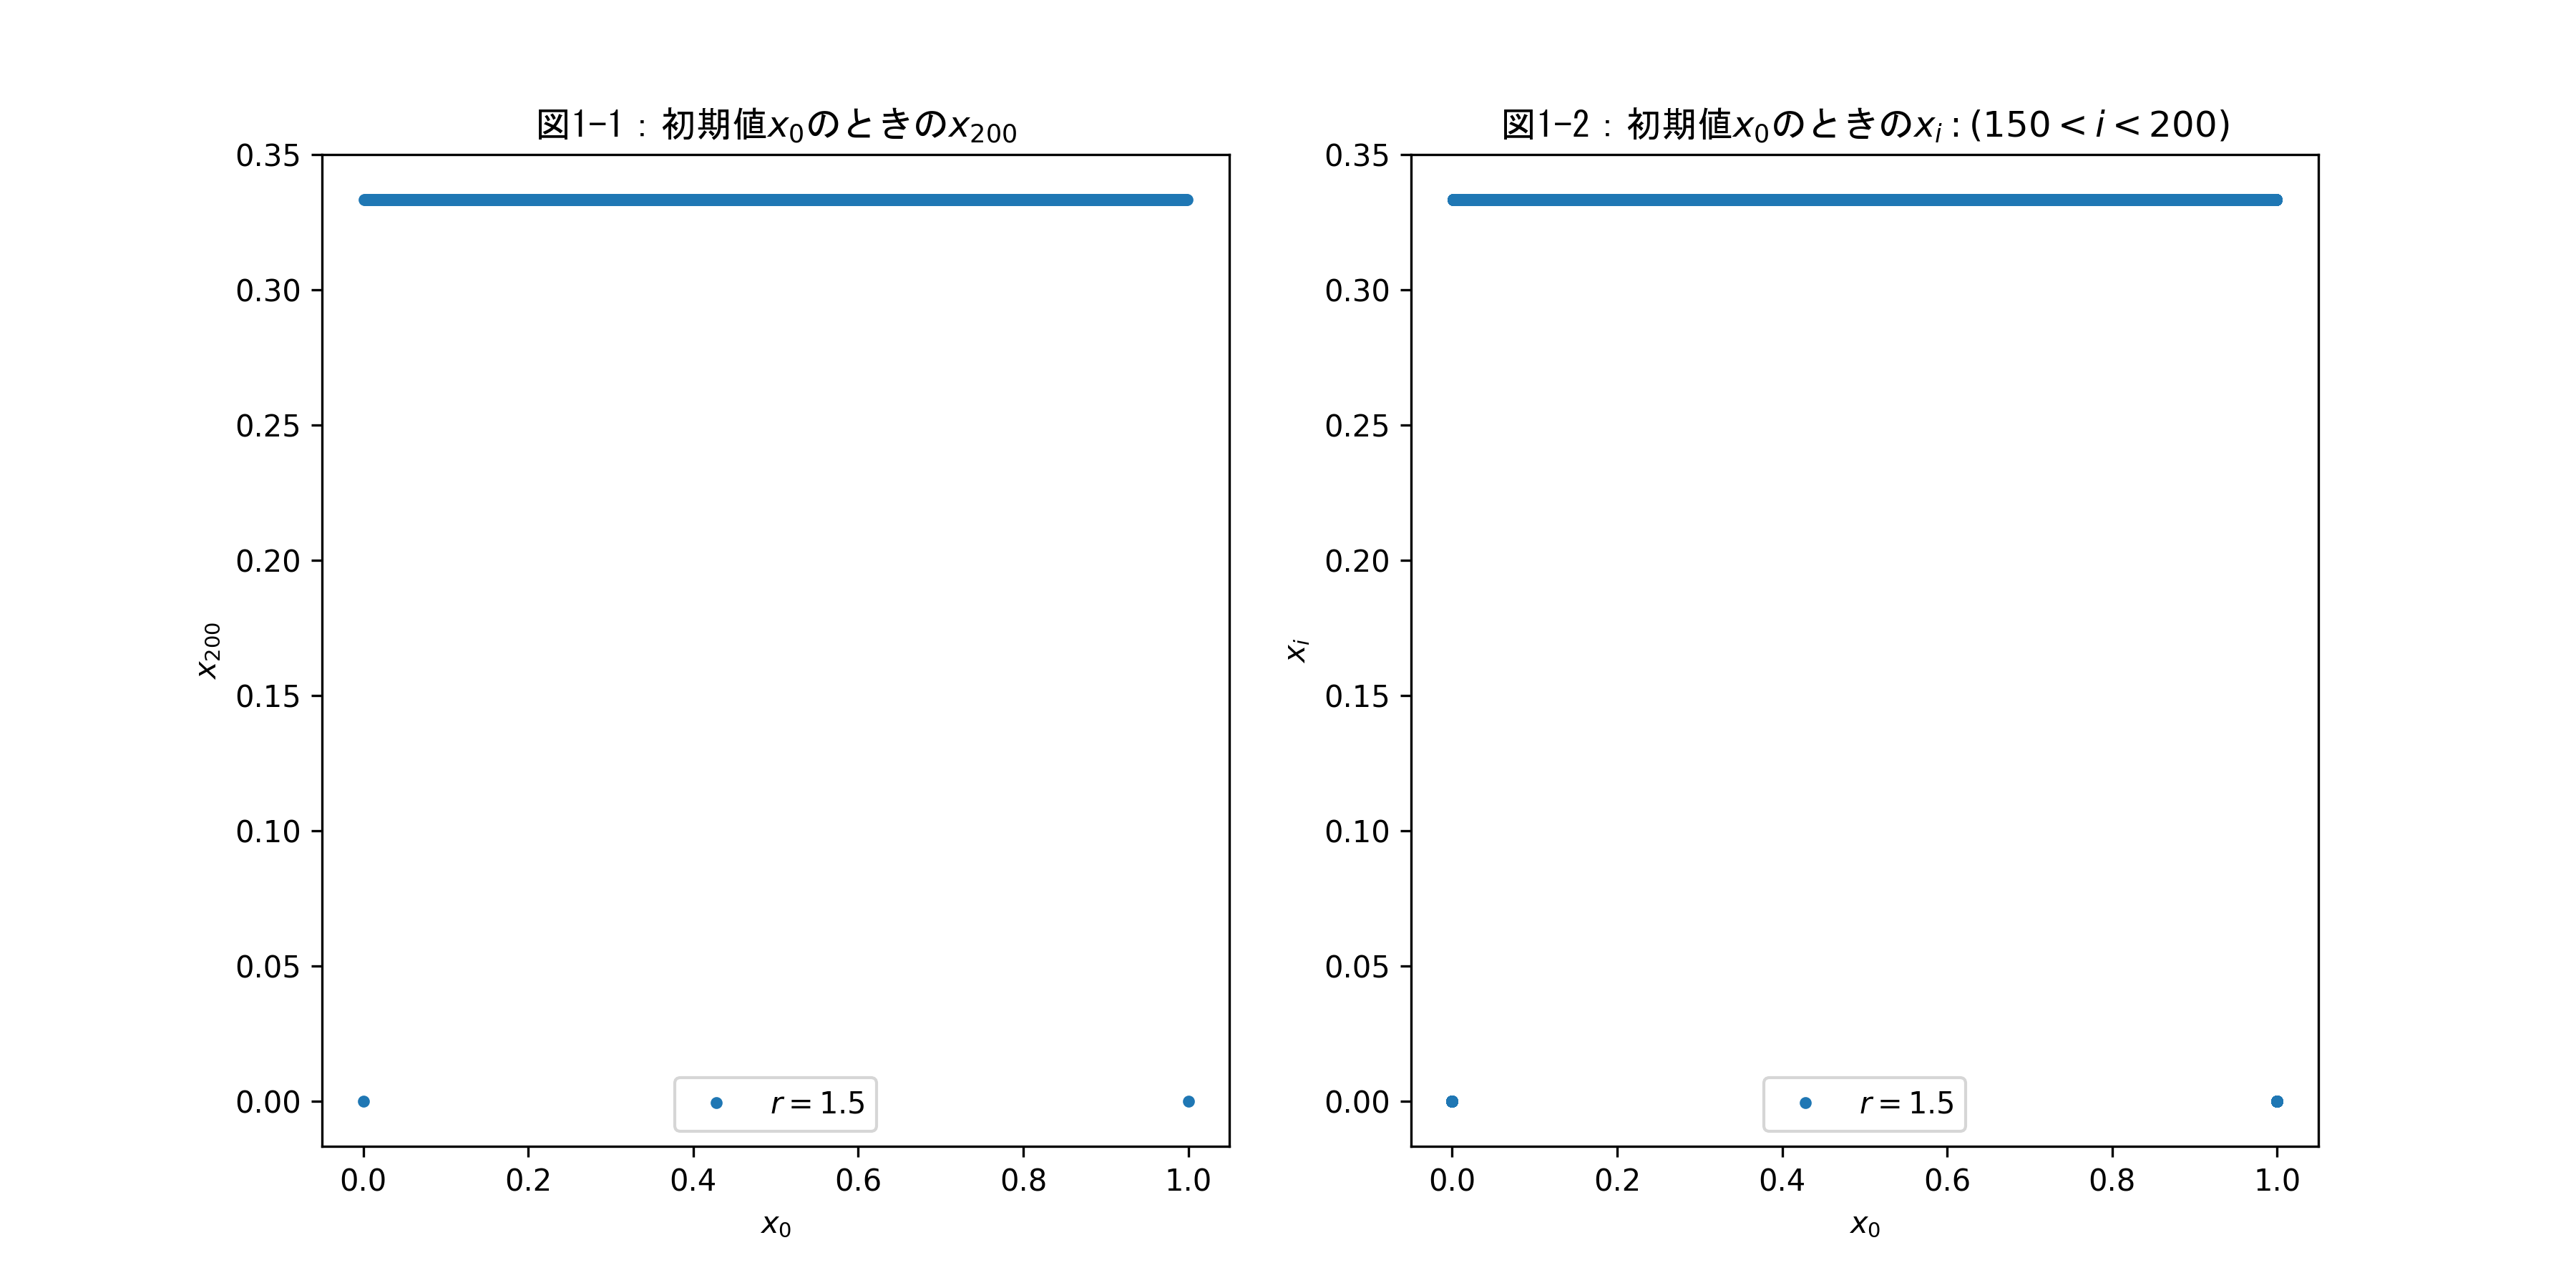
\includegraphics[keepaspectratio, scale=0.25]{images/Problem2/ctest3_1.png}
    \end{minipage} &
    \begin{minipage}[t]{0.45\hsize}
      \centering
      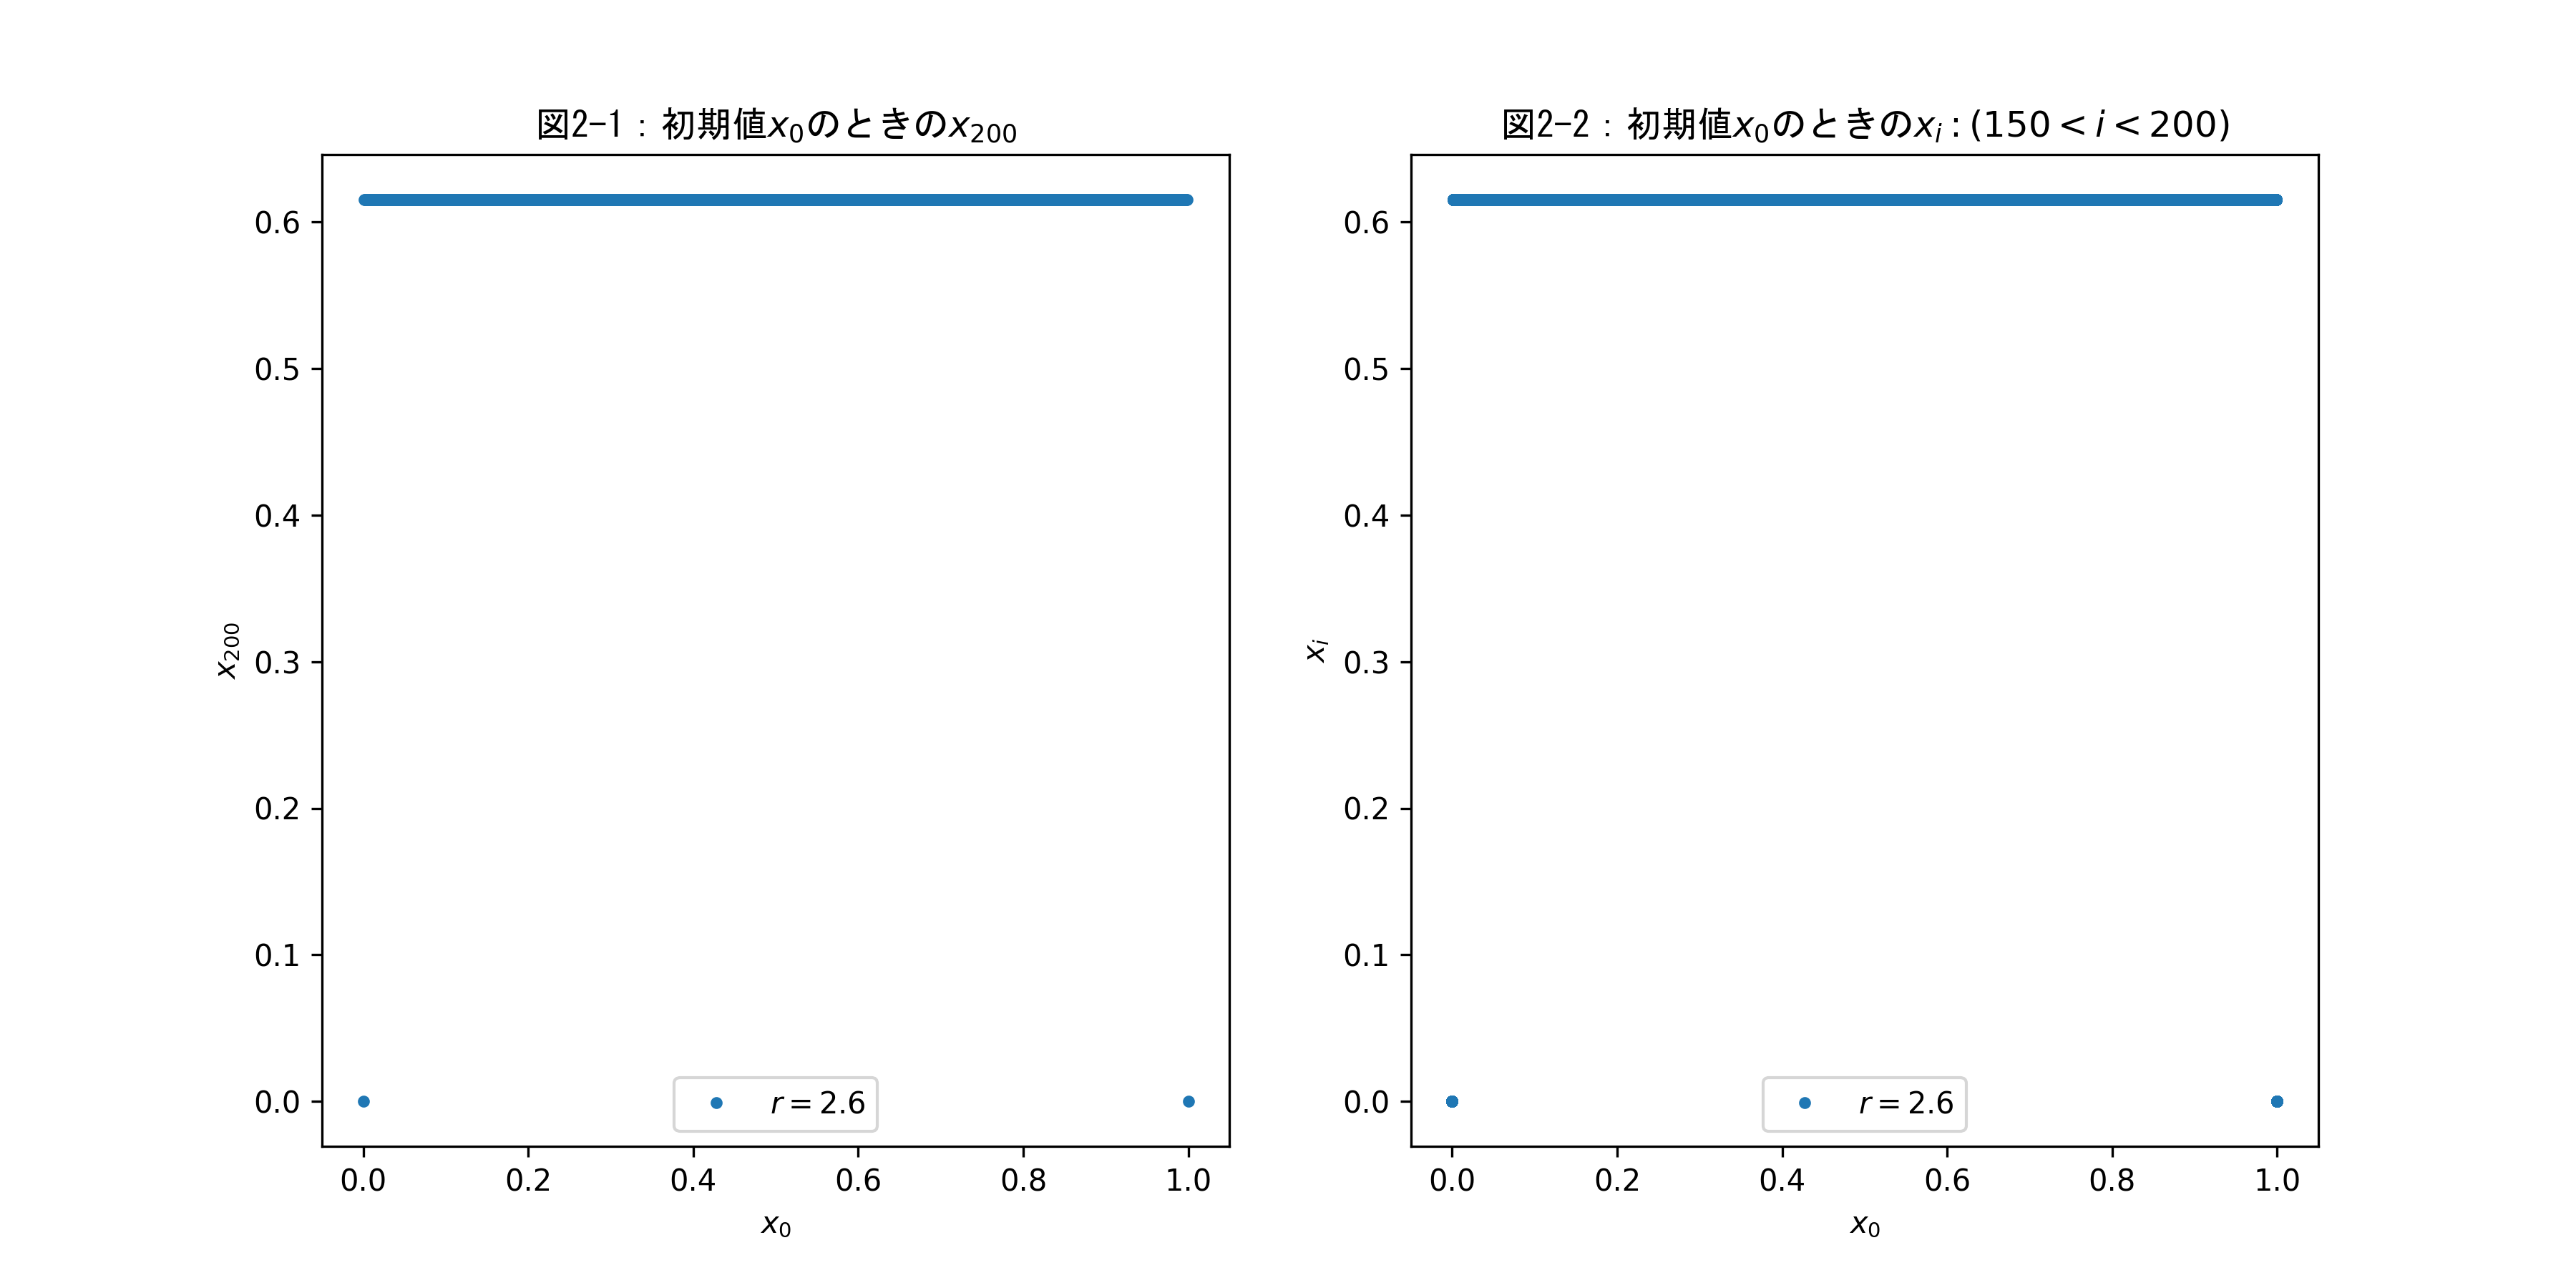
\includegraphics[keepaspectratio, scale=0.25]{images/Problem2/ctest3_2.png}
    \end{minipage} \\

    \begin{minipage}[t]{0.45\hsize}
      \centering
      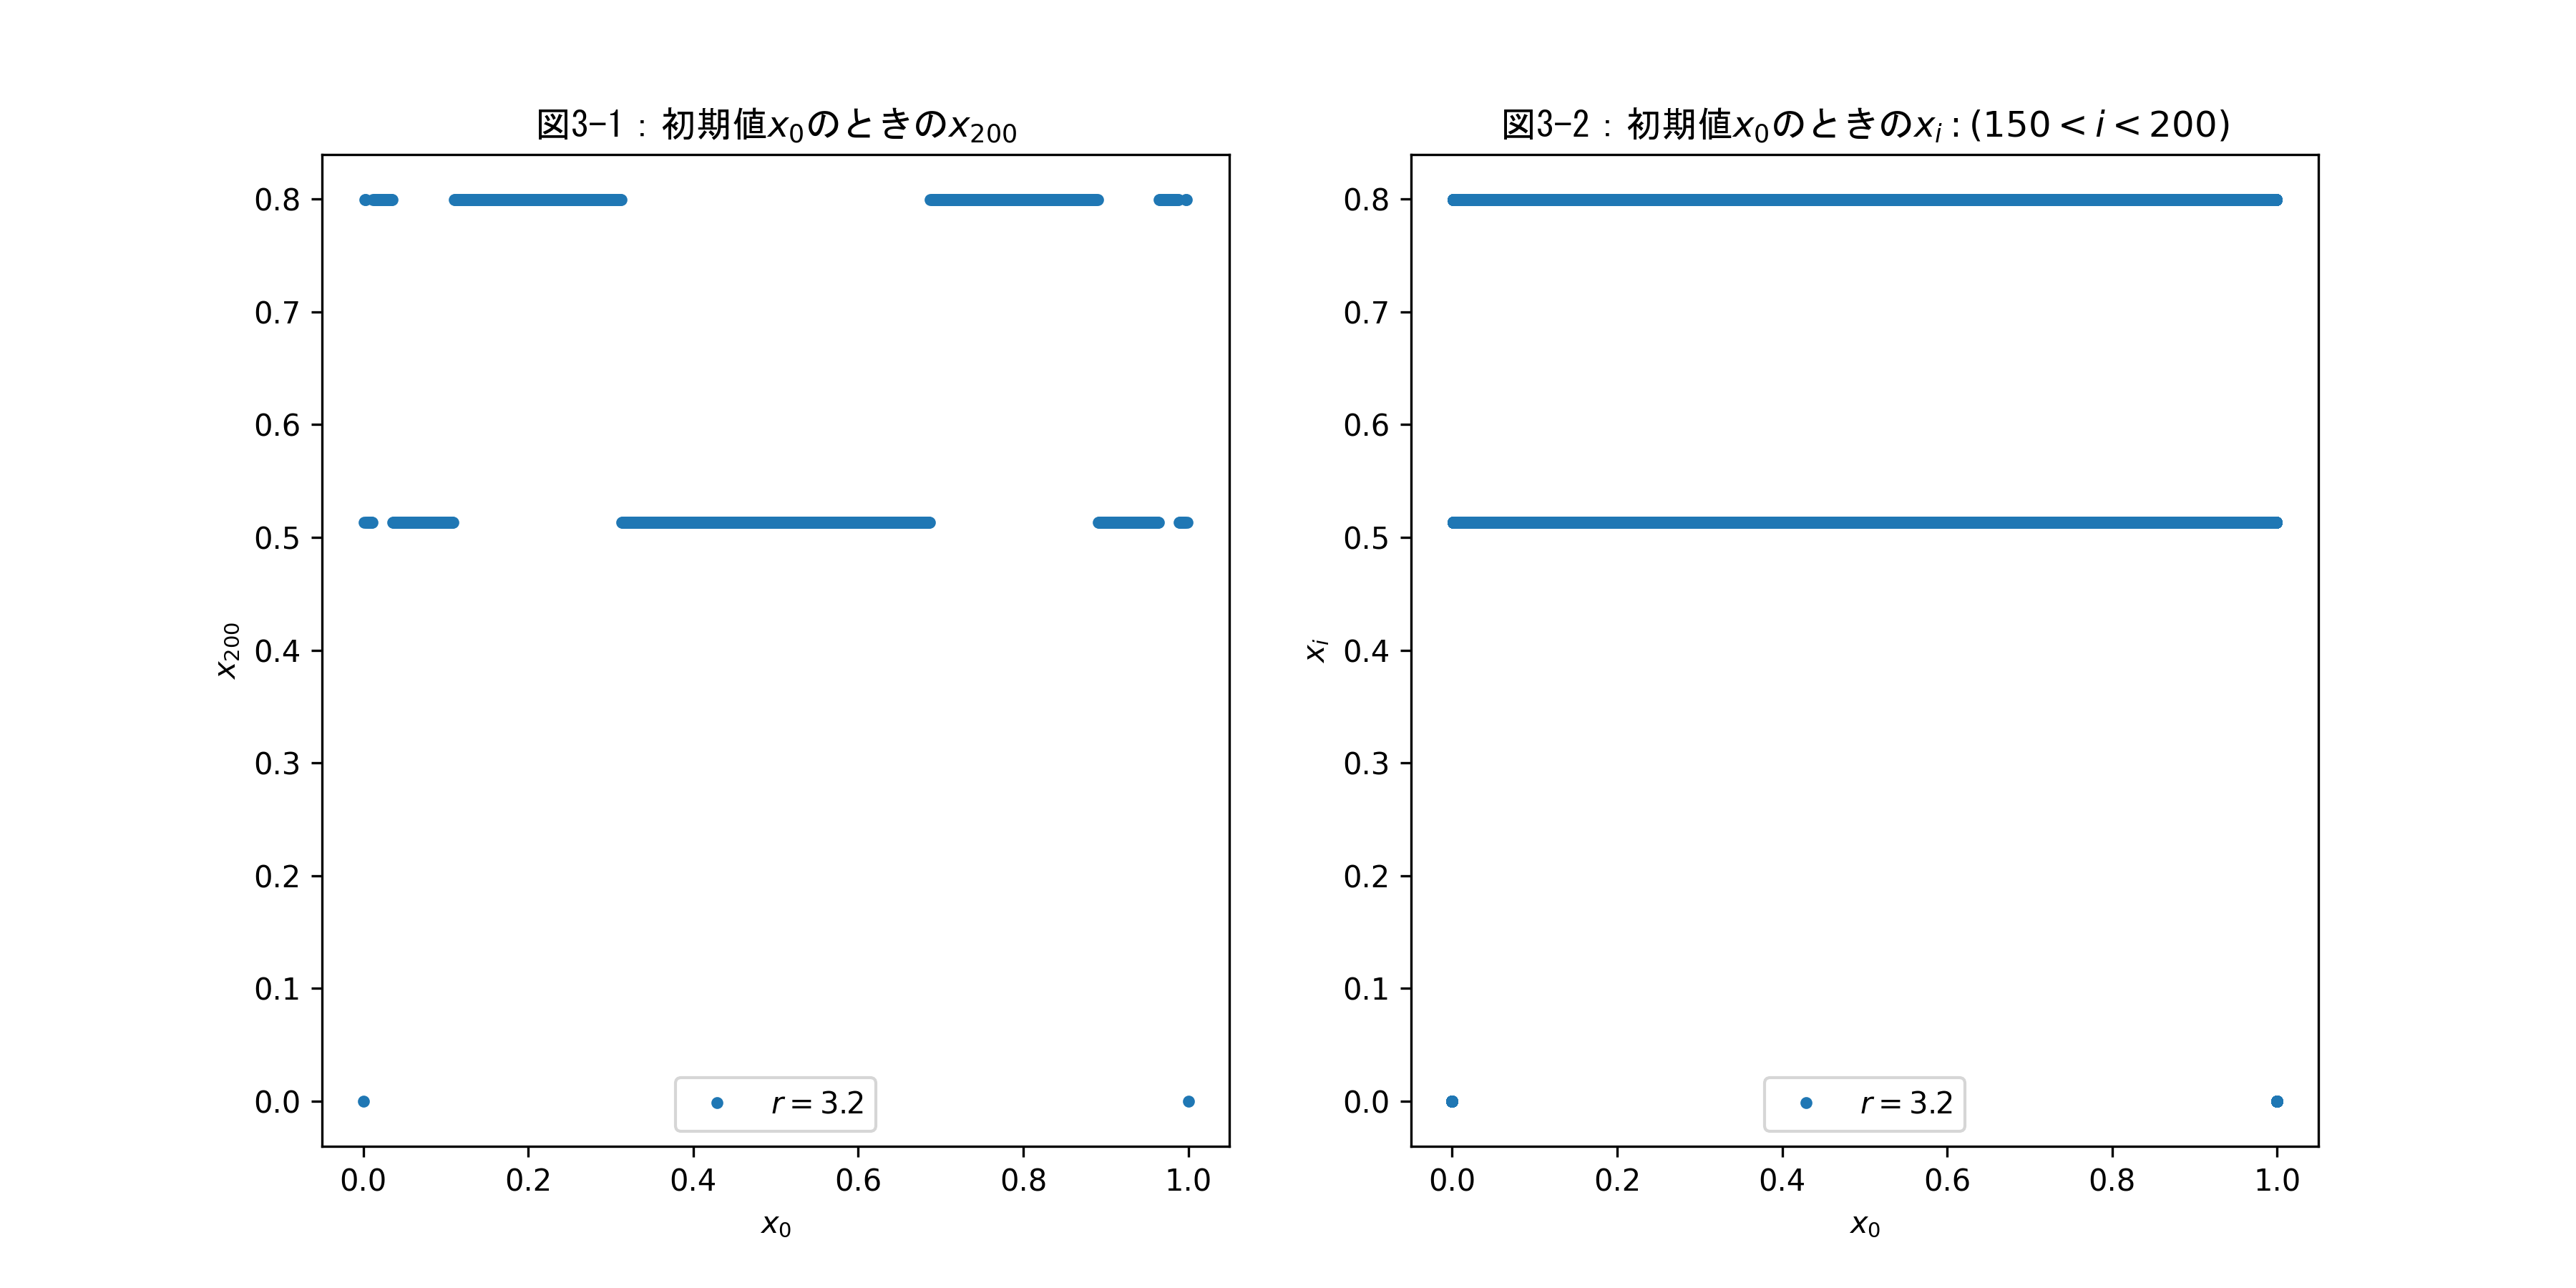
\includegraphics[keepaspectratio, scale=0.25]{images/Problem2/ctest3_3.png}
    \end{minipage} &
    \begin{minipage}[t]{0.45\hsize}
      \centering
      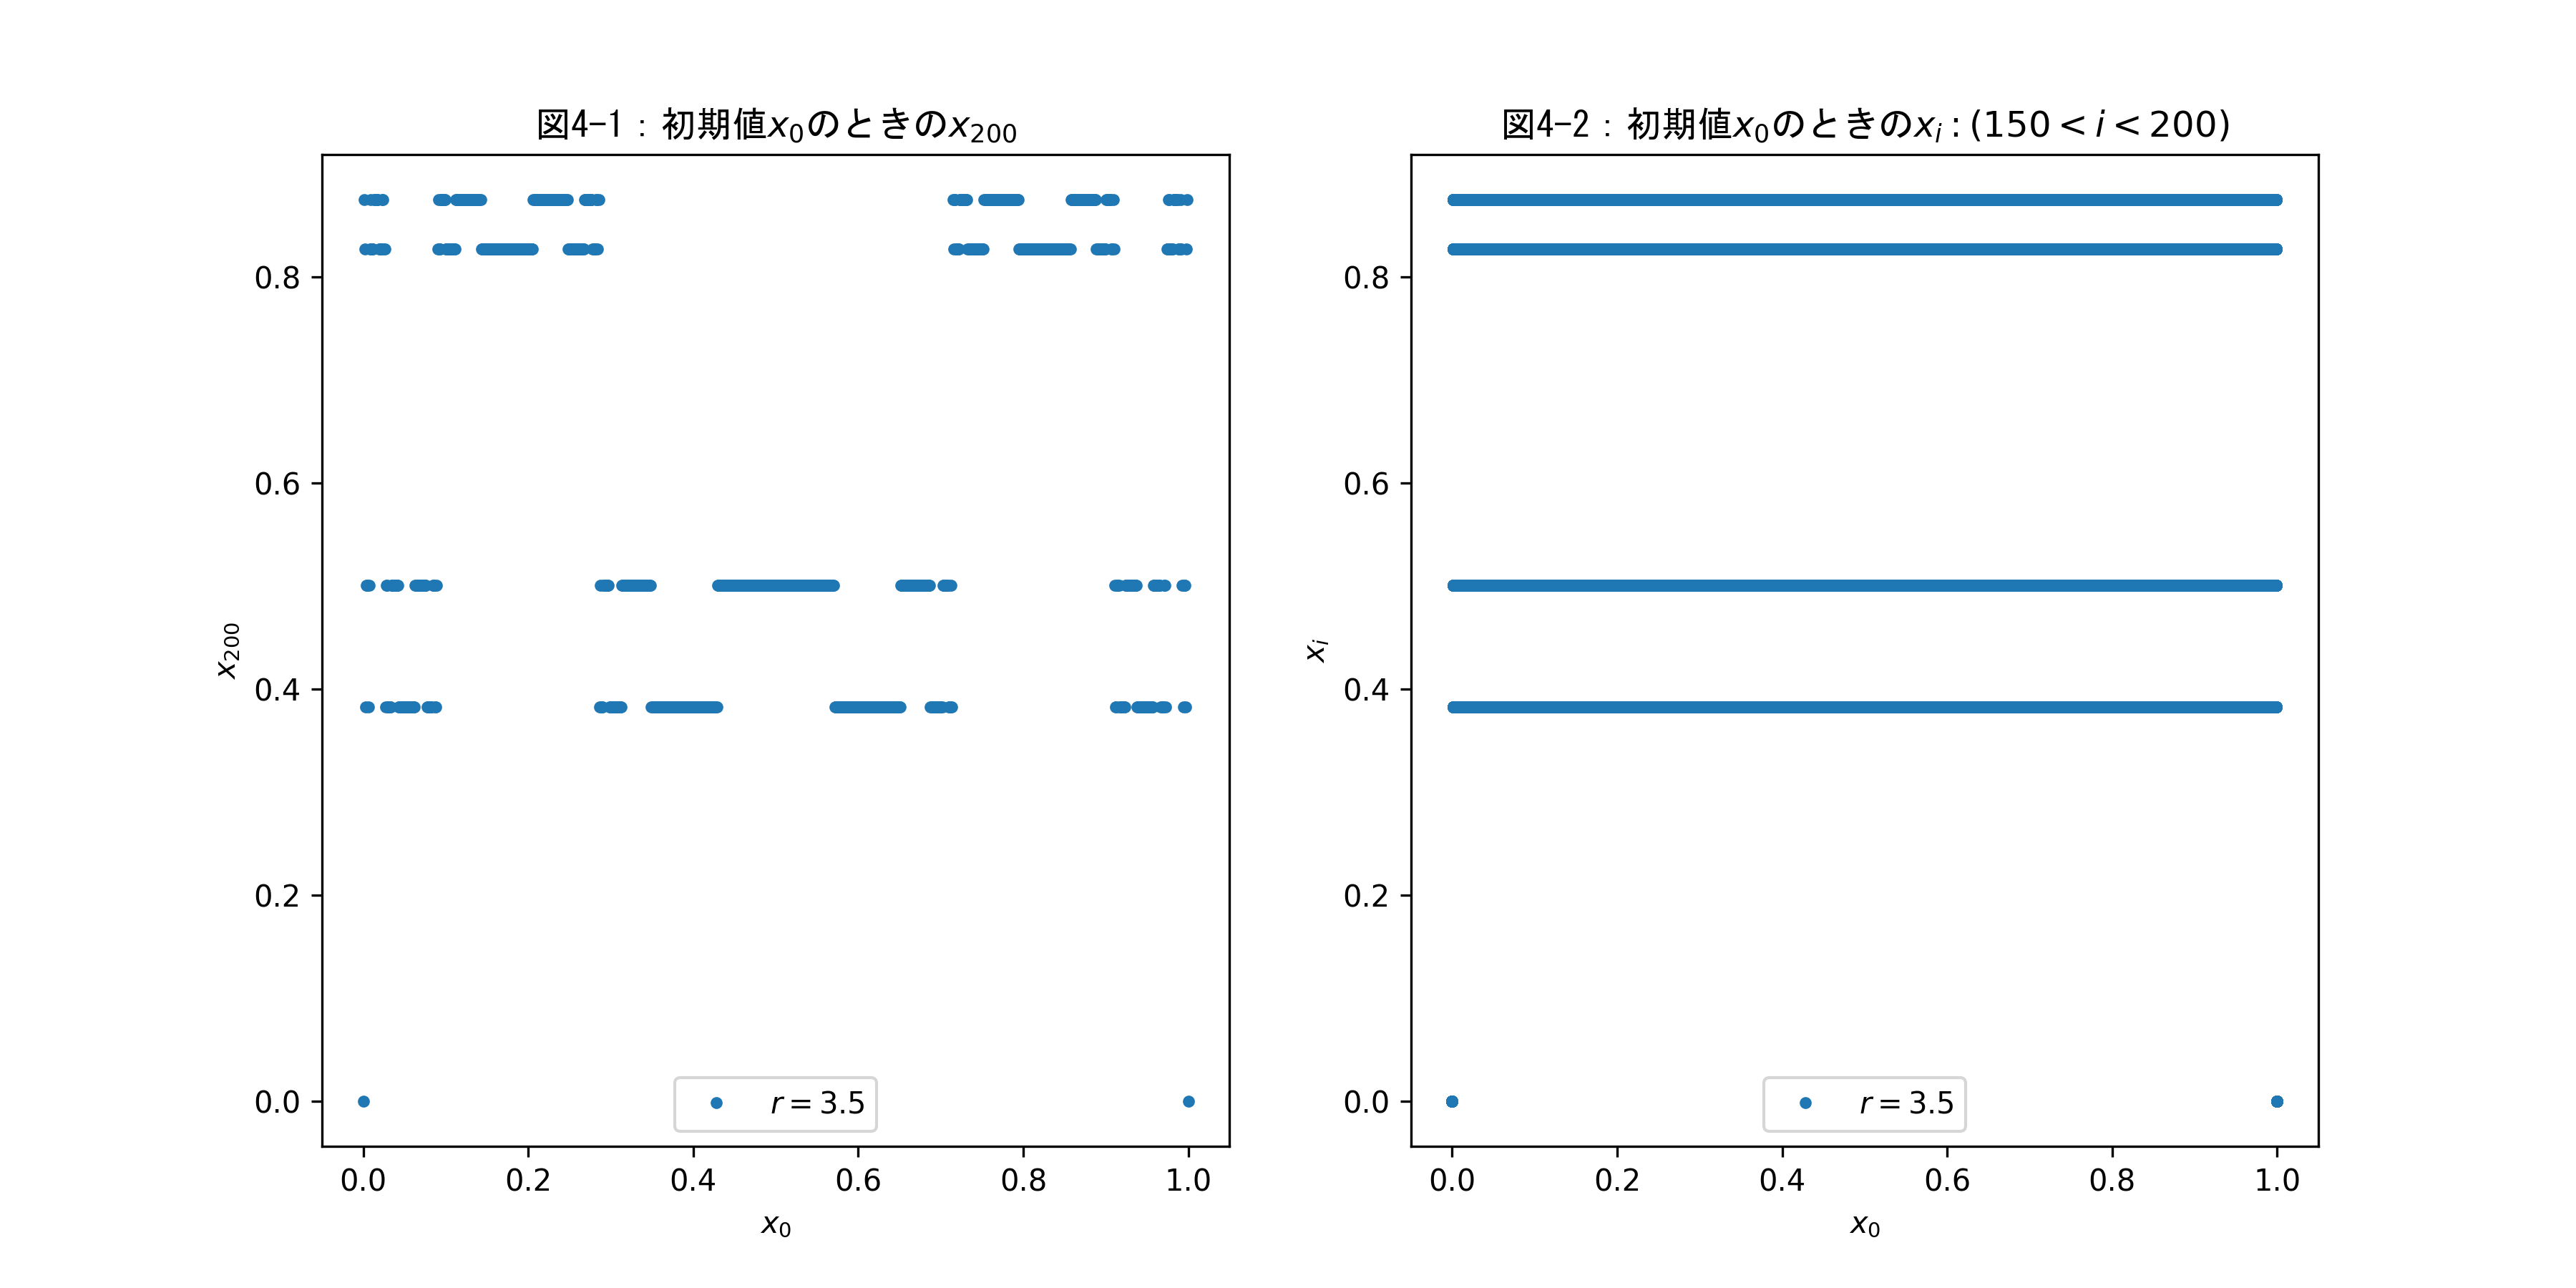
\includegraphics[keepaspectratio, scale=0.25]{images/Problem2/ctest3_4.png}
    \end{minipage} \\

    \begin{minipage}[t]{0.45\hsize}
      \centering
      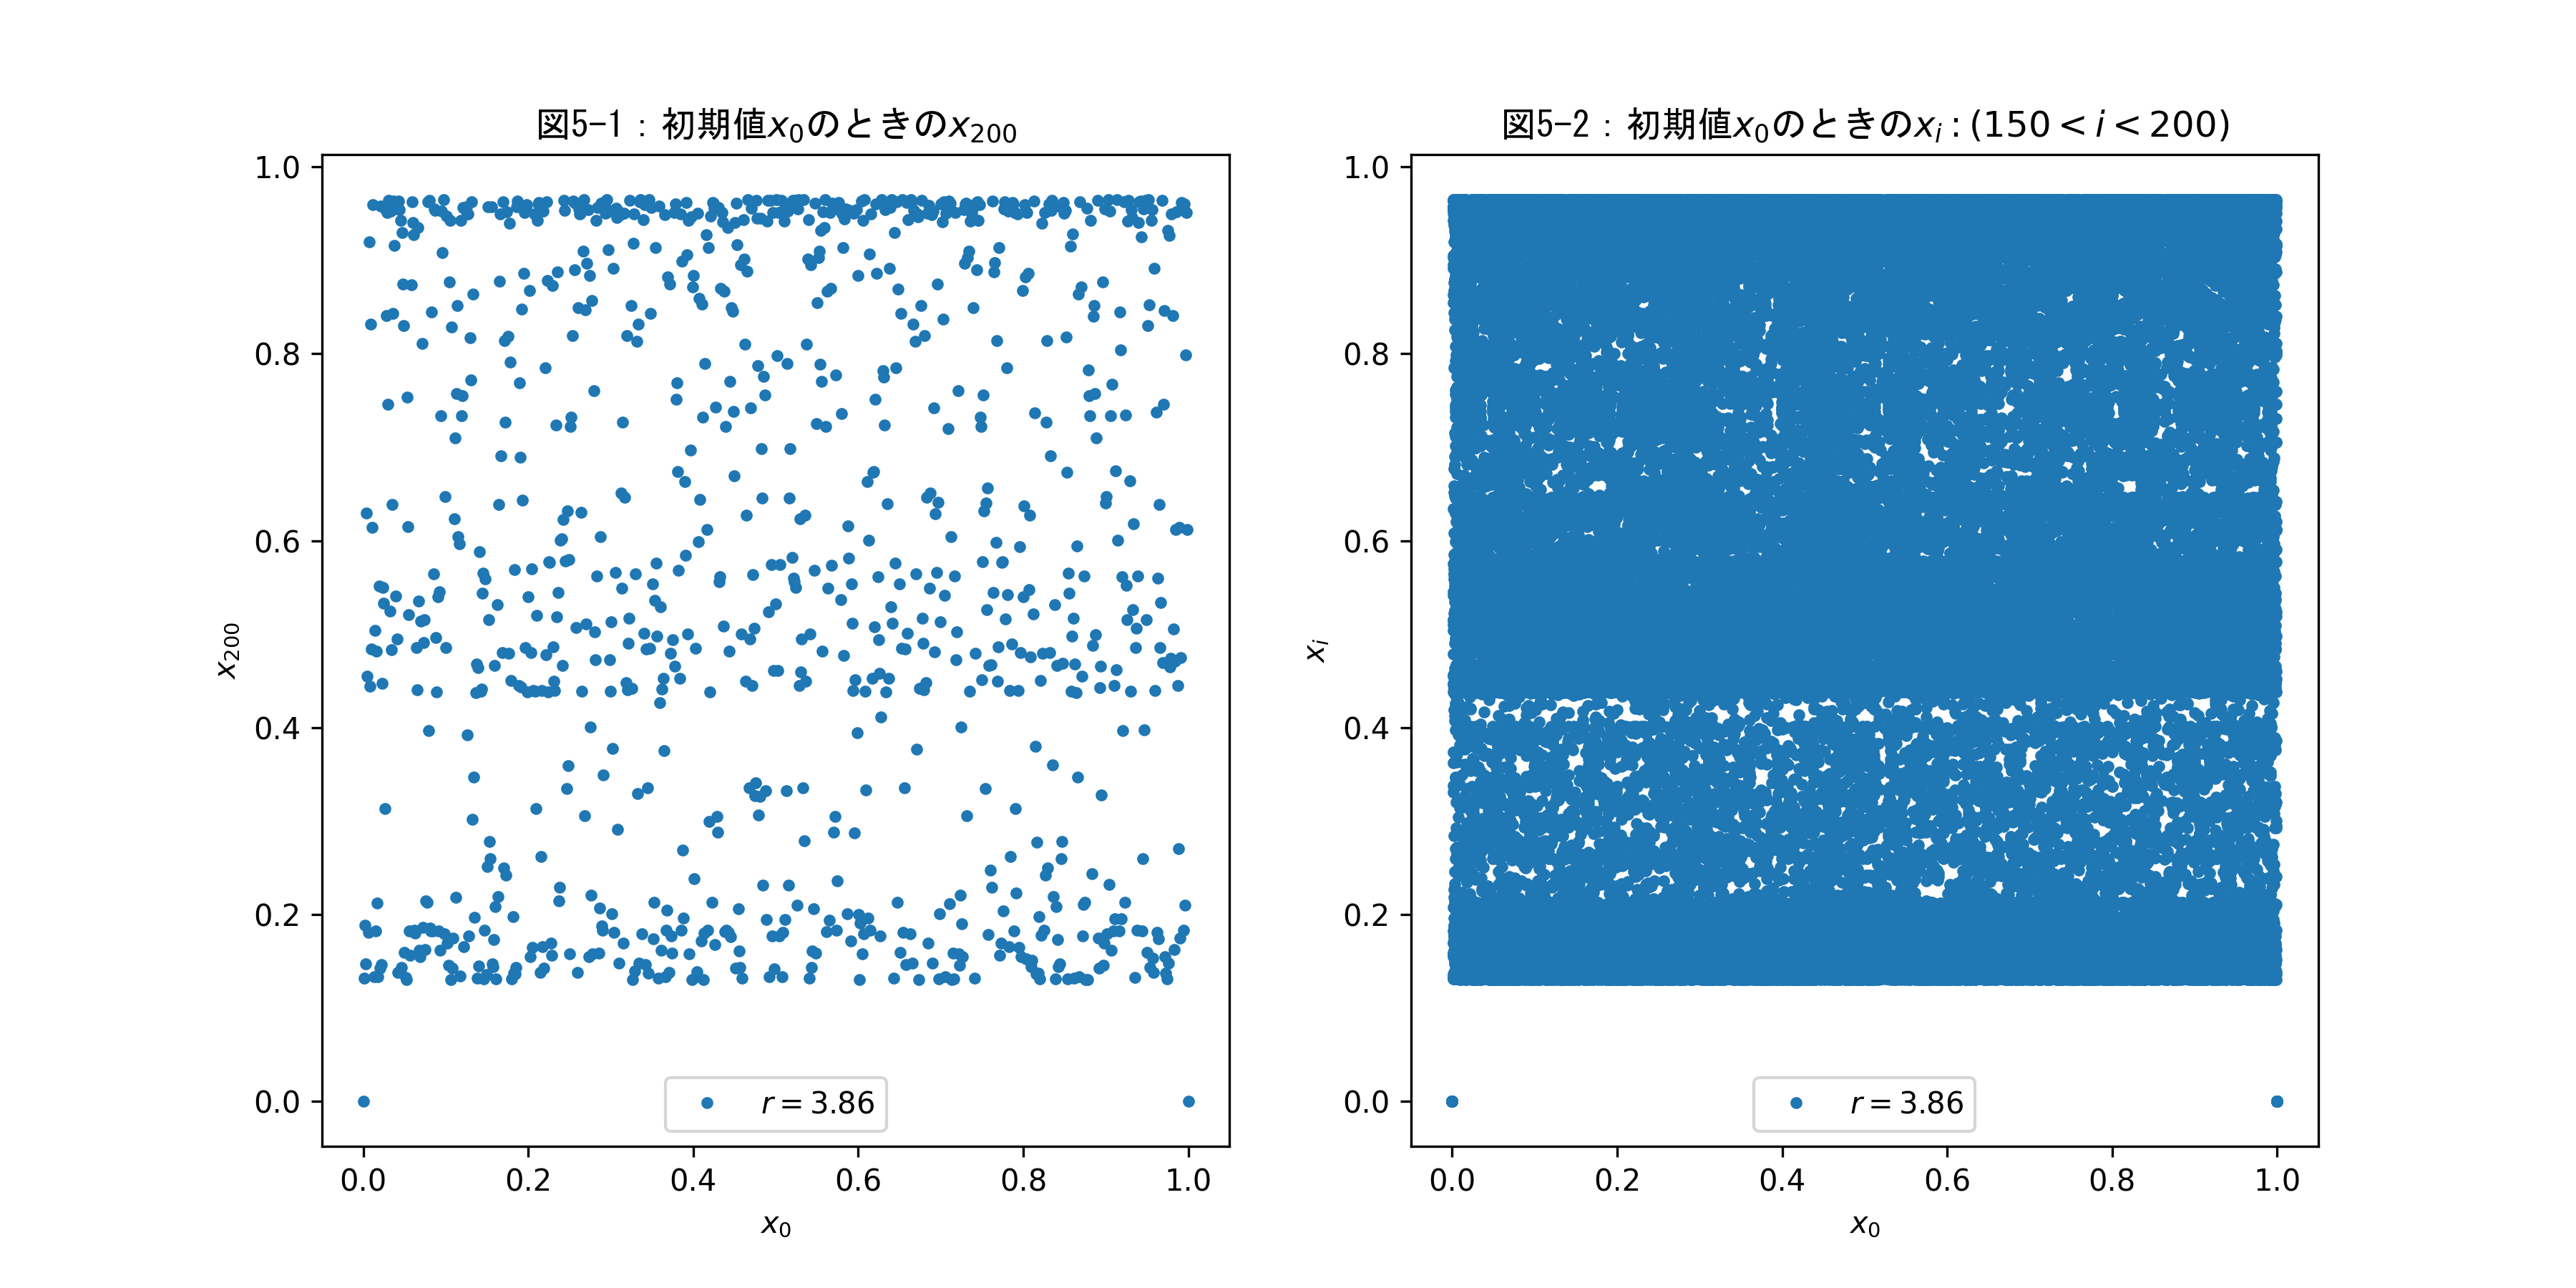
\includegraphics[keepaspectratio, scale=0.25]{images/Problem2/ctest3_5.png}
    \end{minipage} &
    \begin{minipage}[t]{0.45\hsize}
      \centering
      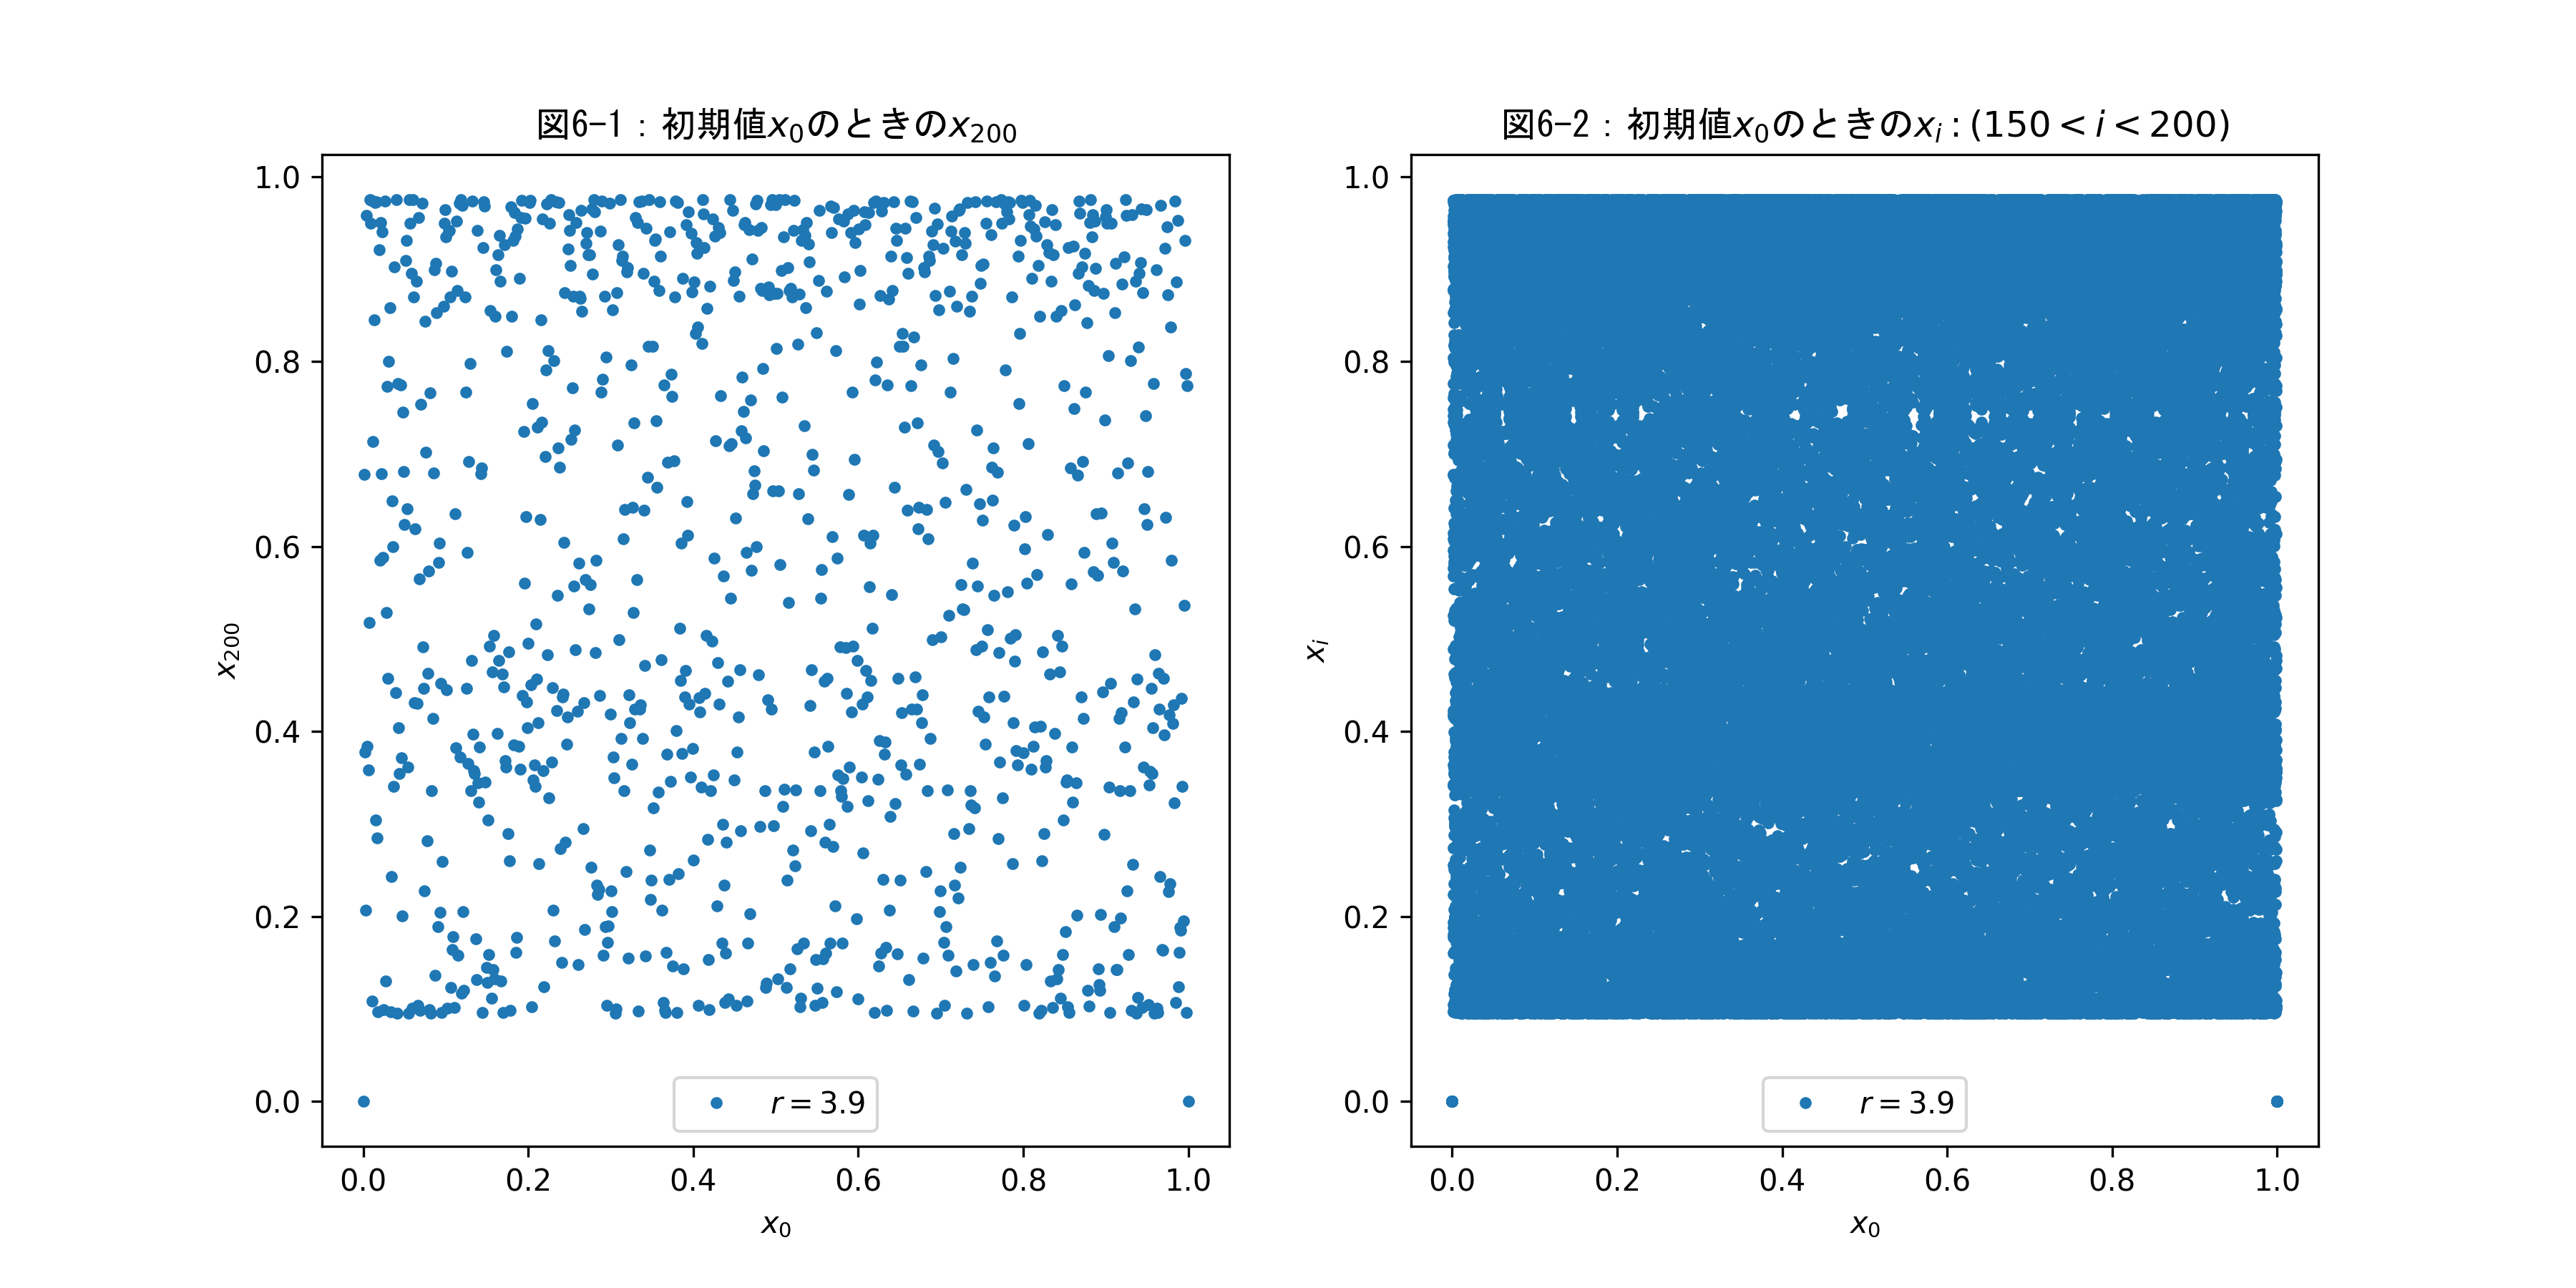
\includegraphics[keepaspectratio, scale=0.25]{images/Problem2/ctest3_6.png}
    \end{minipage}
  \end{tabular}
\end{figure}


結果:\\
$r = 1.50, r = 2.60$ のときは、$x_{200}, x_n (150 < n < 200)$ のどちらも値は一つに定まる。 $r = 3.20$ のときは、 $x_{200}, x_n (150 < n < 200)$ は2通りの値のどちらかに定まることが読み取れる。また、 $r = 3.50$ のときは、 $x_{200}, x_n (150 < n < 200)$ は4通りの値のいづれかに定まる。$r = 3.86, r = 3.90$ のときは、 $x_{200}, x_n (150 < n < 200)$ のどちらもある値に定まることはなく、不規則な値を取り続けている。\\\\

考察:\\
これらの結果から、 $r = 3.86, r = 3.90$ のときは初期値 $x_0$ の小さい変化によって$x_{200}$ と $x_n (150 < n < 200)$ が大きく変化することが考察できる。

\subsection{課題2}
課題1で得られた結果から初期値鋭敏性を説明せよ。\\
課題1で得られた結果から考察した際に、「$r = 3.86, r = 3.90$ のときは初期値 $x_0$ の小さい変化によって$x_{200}$ と $x_n (150 < n < 200)$ が大きく変化することが考察できる。」と書いたが、このように初期値の小さい変化である数 $n$ のときの $x_n$ の値が大きく変化することを初期値鋭敏性という。

